%%%%%%%%%%%%%%%%%%%%%%%%%%%%%%%%%%%%%%%%%%%%%%%%%%%%%%%%%%%%%%%%%%%%%%%%%%%%%%%%%%%%%%%%%%%%%%%%%%%%%%%%%%%%%%%%%
% ---------------------------------------- SEÇÃO DO DOCUMENTO ------------------------------------------------- %
%%%%%%%%%%%%%%%%%%%%%%%%%%%%%%%%%%%%%%%%%%%%%%%%%%%%%%%%%%%%%%%%%%%%%%%%%%%%%%%%%%%%%%%%%%%%%%%%%%%%%%%%%%%%%%%%%

\section{Exemplo}
\label{sec:exemplo}

\subsection{Sub-exemplo}
\label{sec:sub-exemplo}

%%%%%%%%%%%%%%%%%%%%%%%%%%%%%%%%%%%%%%%%%%%%%%%%%%%%%%%%%%%%%%%%%%%%%%%%%%%%%%%%%%%%%%%%%%%%%%%%%%%%%%%%%%%%%%%%%
% ----------------------------------------------- MODELOS ----------------------------------------------------- %
%%%%%%%%%%%%%%%%%%%%%%%%%%%%%%%%%%%%%%%%%%%%%%%%%%%%%%%%%%%%%%%%%%%%%%%%%%%%%%%%%%%%%%%%%%%%%%%%%%%%%%%%%%%%%%%%%

\begin{comment}

%%%% ==================== EQUAÇÃO ==================== %%%%

	\begin{equation}
		\label{eq:}
	\end{equation}
	
%%%% ==================== FIGURA ===================== %%%%

\begin{figure}[h!]

	\centering
	\includegraphics[width=\linewidth]{figuras\}
	\caption{xxxxx.}	
	\label{fig:xxx}
	
\end{figure}

\begin{figure}[H]

	\centering
	\caption{Formulação básica por injeções de potência.}
	
	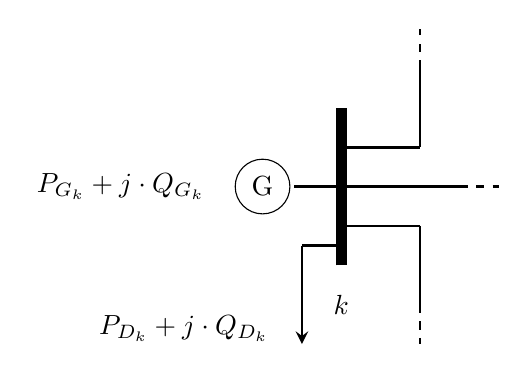
\begin{tikzpicture}
	
		% Imagem 1
		
		\draw node[draw, circle] (no1) at (0., 0.) {G} ;
		
		\draw[line width=4pt] (1., -1.) -- (1., 1.);
		
		\draw[line width=1pt] (0.4, 0.) -- (2.5, 0.);
		
		\draw[line width=1pt] (1., 0.5) -- (2.0, 0.5);
		
		\draw[line width=1pt] (1., -0.5) -- (2.0, -0.5);
		
		\draw[line width=1pt] (2.0, 0.5) -- (2.0, 1.5);
		
		\draw[line width=1pt] (2.0, -0.5) -- (2.0, -1.5);
		
		\draw[dashed, line width=1pt] (2.5, 0.) -- (3., 0.);
		
		\draw[dashed, line width=1pt] (2., 1.5) -- (2., 2.);
		
		\draw[dashed, line width=1pt] (2., -1.5) -- (2., -2.);
		
		\draw[line width=1pt] (0.5, -0.75) -- (1., -0.75);
		
		\draw[->, >=stealth, line width=1pt] (0.5, -0.75) -- (0.5, -2.);
		
		\draw node (no2) at (1., -1.5) {$k$} ;
		
		\draw node (no2) at (-1.8, 0.) {$P_{G_k} + j \cdot Q_{G_k}$} ;
		
		\draw node (no2) at (-1., -1.8) {$P_{D_k} + j \cdot Q_{D_k}$};
		
	\end{tikzpicture}
	
	\label{fig:}	
	
\end{figure}

\begin{figure}[H]

	\centering
	\caption{Desenho exemplo.}
	
	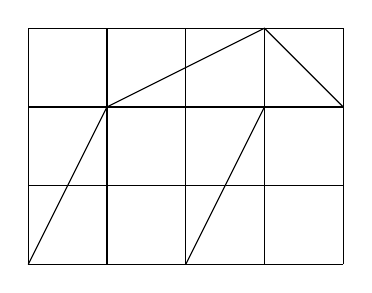
\begin{tikzpicture}
	
		\draw (0,0) grid (4,3);
		\draw (0,0) -- (1,2) -- (3,3) -- (4,2);
		\draw (2,0) -- (3,2);
	
	\end{tikzpicture}
	
	\label{fig:}	

\end{figure}


%%%% ===================== TABELA ==================== %%%%

\begin{table}[h!]
	\centering
	\caption{xxx}
	\label{tab:xxx}
	\begin{tabular}{|c|c|}
	\end{tabular}  
\end{table}


\end{comment}